\chapter{Lattice gauge theory}
\label{chap:latticeqcd}

\section{Gauge invariance} 
Nevertheless, a naive discretization of the Yang-Mills action from Equation \cref{yangmills}, in which one replaces all the partial derivatives appearing in the field strengths $F^{\mu\nu}$ with finite differences leads to the loss of gauge invariance \cite{schwartz, peskin}. 

\begin{remark}
This is a consequence of imposing local gauge symmetry, with a $\textsf{SU}(3)$ gauge transformation given by Equation \cref{gaugetransf}, of the fields
\begin{align*}
    \phi(x)\mapsto \textsf{U}(x)\phi(x).
\end{align*}
Fields at different space-time points cannot directly be compared. Because of this, the partial derivative, which contains the difference between fields at different points, is not well defined. By introducing a quantity which gauge transform as
\begin{align}\label{latt3}
    \textsf{W}(x,y)\mapsto\textsf{U}(x)\textsf{W}(x,y)\textsf{U}^\dagger(y),
\end{align}
one may now properly define the covariant derivative as\footnote{Notice that with this definition, the covariant derivative transforms as
\begin{align}\label{latt1}
    \textsf{D}_\mu\phi(x)\mapsto\textsf{U}(x)\textsf{D}_\mu\phi(x).
\end{align}
}

\begin{definition}[Covariant derivative]
\begin{align}\label{latt2}
    \textsf{D}_{\mu} \phi(x)\overset{\Delta}{=} \lim _{\delta \epsilon^{\mu} \rightarrow 0} \frac{\textsf{W}(x, x+\epsilon) \phi(x+\epsilon)-\phi(x)}{\epsilon^\mu}.
\end{align}
\end{definition}
\noindent We choose $\textsf{W}(x,x)=\mathds{1}$ and then write an expansion in terms of the gauge fields\footnote{If we plug in this relation back in Equation \cref{latt2} and then in Equation \cref{latt1}, we deduce the gauge transformation of the gauge fields from Equation \cref{gaugefields}.}
\begin{align*}
    \textsf{W}(x,x+\epsilon)=1+ig\epsilon^\mu A_\mu+\mathcal{O}(\epsilon^2).
\end{align*}
\end{remark}

This enables us to express the {\sffamily\color{maincolor}Wilson line} as\footnote{Where the fields may further be written as $A_{\mu}=A_{\mu}^aT^a$ in the fundamental representation.}
\boxedeqlabel{latt5}{
    \textsf{W}(x,y)=\mathcal{P}\exp{i g \int_{y}^{x} \mathrm{d} z^{\mu} A_{\mu}(z) }
}

\begin{remark}
The {\sffamily\color{maincolor}path-ordering} operator $\mathcal{P}\{\ldots\}$ is necessary due to the non-Abelian nature of the fields. More clearly, after writing a Taylor expansion, the path-ordering operator acts as

\begin{align*}
    \begin{aligned}
    \textsf{W}(x, y)=& 1+i g \int_{0}^{1} \frac{\mathrm{d} z^{\mu}_\lambda}{\mathrm{d} \lambda} A_{\mu}^{a}(z_\lambda^\mu) T^{a} \mathrm{d} \lambda-\frac{1}{2} g^{2} \int_{0}^{1} \mathrm{d} \lambda \int_{0}^{1} \mathrm{d} \tau \frac{\mathrm{d} z^{\mu}_\lambda}{\mathrm{d} \lambda} \frac{\mathrm{d} z^{\nu}_\tau}{\mathrm{d} \tau}\times\\
    & \times A_{\mu}^{a}(z_\lambda^\mu) A_{\nu}^{b}(z_\tau^\nu)\left[T^{a} T^{b} \theta(\lambda-\tau)+T^{b} T^{a} \theta(\tau-\lambda)\right]+\cdots.
\end{aligned}
\end{align*}
\end{remark}

A Wilson line taken along a closed path $\gamma$ is called a {\sffamily\color{maincolor}Wilson loop} and it's given by
\boxedeqlabel{latt4}{
    \textsf{W}_\gamma=\mathcal{P}\exp{i g \oint\limits_{\gamma} \mathrm{d} x^{\mu} A_{\mu}(x)}
}

It is important to emphasize that the trace of a Wilson loop is gauge invariant\footnote{This may easily be proven by inserting Equation \cref{latt4} back in Equation \cref{latt3} and using the invariance of the trace under cyclic permutations.}.

\section{Real-time lattice gauge theory} 
Let us begin by discretizing the Minkowski space-time on a hypercubic lattice\footnote{The lattice spacing along direction $\mu$, with the unit vector is $\hat{e}^\mu$, is $a^\mu$. This enables us to write $\hat{a}^{\mu}=a^\mu\hat{e}^\mu$. More concisely, $a^0$ is the time step and $a^i$ denote the spatial lattice spacings.} whose points are given by
\begin{align*}
    \textsf{X}^4=\left\{x \mid x=\sum_{\mu=0}^{3} n_{\mu} \hat{a}^{\mu}, \quad n_{\mu} \in \mathbb{Z}\right\}.
\end{align*}

A field $\phi(x)$ which resides on the lattice will be denoted as $\phi_x$, with $x\in\textsf{X}^4$. The gauge transformation $\textsf{U}(x)$ will become, upon discretization, $\textsf{U}_x$. The discretized action and corresponding field equations written in terms of $A_\mu$ will not remain gauge invariant.

Nevertheless, a gauge invariant lattice action may be constructed. Instead of using the gauge fields $A_\mu$, along with the corresponding conjugate momenta $P_\mu$, as the main degrees of freedom, one may simply seek for a more suitable quantity which is already gauge invariant and preserves gauge invariance upon discretization. An action built from such a quantity will inherently be gauge invariant. The simplest choice is the trace of a Wilson line, as given in Equation \cref{latt4}. We already saw that such a construction is gauge invariant.

\begin{figure}
    \centering
    \subfloat[\centering {\sffamily 2d} plaquette]{{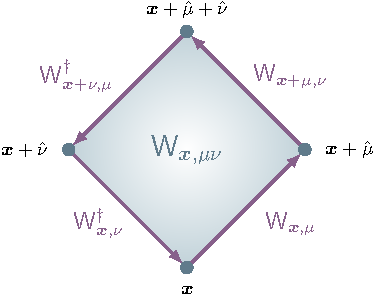
\includegraphics[width=0.45\textwidth]{plaquette_2d.pdf} }}%
    \qquad
    \subfloat[\centering {\sffamily 3d} plaquette]{{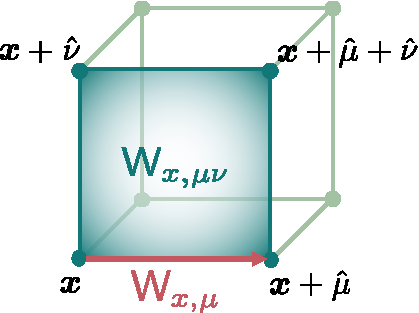
\includegraphics[width=0.45\textwidth]{plaquette_3d.pdf} }}%
    \caption{Schematic representations of a plaquette, the shortest Wilson loop on a rectangular lattice.}%
    \label{fig:plaquettes}%
\end{figure}

A Wilson line taken between two neighboring lattice points, namely $x$ and $x+\hat{a}^{\mu}$, is called a {\sffamily\color{maincolor}gauge link} and it's given by\footnote{Here $\overline{\mathcal{P}}\{\ldots\}$ denotes the anti-path-ordering. We introduce the notation
\begin{align*}
    \textsf{W}_{x,\mu}\overset{\Delta}{=}\textsf{W}(x,x+\hat{a}^{\mu})
\end{align*}
and similarly for $A_{x,\mu}$.
}
\begin{align*}
    \textsf{W}_{x, \mu}=\overline{\mathcal{P}} \exp{i g \int\limits_{x}^{x+\hat{a}^{\mu}} d x^{\mu} A_{x,\mu}}.
\end{align*}

\begin{remark}
In a similar manner, we may also introduce a gauge link along the opposite direction, which would yield
\begin{align}\label{latt6}
    W_{x,\mu}^{\dagger}=\textsf{W}_{x+\mu,-\mu}.
\end{align}
A gauge link transforms as
\begin{align*}
    \textsf{W}_{x, \mu} \rightarrow \textsf{U}_{x} \textsf{W}_{x, \mu} \textsf{U}_{x+\mu}^{\dagger}.
\end{align*}
One may express a gauge link and afterwards expand it, see Equation \cref{latt5}, as
\begin{equation*}
    \begin{aligned}
     \textsf{W}_{x,\mu}&=\exp{iga^\mu A_{x,\mu}}\approx \mathds{1}+iga^\mu A_{x,\mu(x)}-\frac{1}{2}g^2a^\mu a^\nu A_{x,\mu}A_
     {x,\nu}+\mathcal{O}(a^3).
\end{aligned}
\end{equation*}
\end{remark}

The simplest non-trivial\footnote{The shortest Wilson line would just go back and forth between two neighbouring sites but such a combination would simply yield the trivial result
\begin{align*}
    \textsf{W}_{x,\mu}\textsf{W}_{x+\mu,-\mu}\stackrel{\text{\cref{latt6}}}{=\joinrel=}\mathds{1}.
\end{align*}
} Wilson loop on the lattice may be constructed along the path connecting neighbouring points on a rectangular {\sffamily\color{maincolor}plaquette}, see Figure \cref{fig:plaquettes}, as
\begin{align*}
    \textsf{W}_{x, \mu \nu}&=\textsf{W}_{x, \mu} \textsf{W}_{x+\mu, \nu} \textsf{W}^\dagger_{x+\mu,\mu}\textsf{W}^\dagger_{x,\nu}\\
    &\stackrel{\text{\cref{latt6}}}{=\joinrel=}\textsf{W}_{x, \mu} \textsf{W}_{x+\mu, \nu} \textsf{W}_{x+\mu+\nu,-\mu} \textsf{W}_{x+\nu,-\nu},
\end{align*}
which may further be expressed as
\begin{align*}
    \textsf{W}_{x, \mu \nu} \approx \exp{ig a^{\mu} a^{\nu} F_{x,\mu \nu}+\mathcal{O}\left(a^{3}\right)}.
\end{align*}

\begin{proof}
We may write the discretized Wilson loop as\footnote{
Using the Campbell-Baker-Hausdorff formula
\begin{align*}
    \exp{\textsf{A}}\exp{\textsf{B}}\approx\exp{\textsf{A}+\textsf{B}+\frac{1}{2}[\textsf{A}, \textsf{B}]+\cdots}.
\end{align*}
}
\begin{align*}
    \textsf{W}_{x,\mu\nu}&\approx\exp\Bigg\{ig(A_{x,\mu}+A_{x+\mu,\nu}-A_{x+\nu,\mu}-A_{x,\nu})+\\
    &\phantom{\approx\exp\Bigg\{}+\frac{g^2}{2}\Big(\big[A_{x,\nu}+A_{x+\nu,\mu},A_{x+\mu,\nu}+A_{x,\mu}\big]-\\
    &\phantom{\approx\exp\Bigg\{}-\big[A_{x,\nu},A_{x+\nu,\mu}\big]-\big[A_{x+\mu,\nu},A_{x,\mu}\big]\Big)\Bigg\}.
\end{align*}
By making use of the expansion 
\begin{align*}
    A_{x+\mu,\nu}\approx A_{x,\nu}+a^\mu\partial_\mu A_{x,\nu}+\mathcal{O}(a^2),   
\end{align*}
we may then derive
\begin{align*}
     \textsf{W}_{x,\mu\nu}&\approx\exp\Big\{iga^\mu a^\nu\underbrace{\big(\partial_\mu A_{x,\nu}-\partial_\nu A_{x,\mu}-ig[A_{x,\nu},A_{x,\mu}]\big)}_{\mathclap{\textstyle F_{x,\mu\nu}}}+\mathcal{O}(a^3)\Big\}.
\end{align*}
This may further be approximated as
\begin{align*}
    \textsf{W}_{x,\mu\nu}=\mathds{1}+ig a^\mu a^\nu F_{x,\mu \nu}-\frac{1}{2}(ga^\mu a^\nu)^2 F_{x,\mu \nu}^2+\mathcal{O}(a^5).
\end{align*}
in the limit of small lattice spacings.
\end{proof}

Therefore, we may construct a gauge invariant quantity, since in contains Wilson lines traced over, under the discretized gauge transformation $\textsf{U}_x$ as

\begin{align}\label{latt7}
    \textsf{Tr}\big\{2-\textsf{W}_{x, \mu \nu}-\textsf{W}_{x, \mu \nu}^{\dagger}\big\} \approx\left(g a^{\mu} a^{\nu}\right)^{2} \textsf{Tr}\big\{F_{x,\mu \nu}^{2}\big\}+\mathcal{O}(a^{6}).
\end{align}

The Yang-Mills action from Equation \cref{yangmills} may be split into an electric and a magnetic part
\begin{align*}
    \textsf{S}=\underbrace{\int \mathrm{d}^{4}x \sum_{i}\textsf{Tr}\big\{F_{0i}^2(x)\big\}}_{\mathclap{\textstyle \textsf{S}_\textsf{E}}}+\underbrace{\int \mathrm{d}^{4}x\sum_{i, j} \frac{1}{2} \textsf{Tr}\big\{F_{ij}^2(x)\big\}}_{\mathclap{\textstyle \textsf{S}_\textsf{B}}}.
\end{align*}
Upon discretization, they become\footnote{By making the replacement
\begin{align*}
    \int \mathrm{d}^{4}x(\ldots)\mapsto \underbrace{\prod\limits_{\mu}a^\mu}_{\mathclap{\textstyle \textsf{V}}}\sum_x(\ldots)
\end{align*}
and using the result from Equation \cref{latt7}.
}
\begin{align*}
    \textsf{S}_\textsf{E}& \approx V \sum_{x} \sum_{i} \frac{1}{\left(g a^{0} a^{i}\right)^{2}} \textsf{Tr}\big\{2-\textsf{W}_{x, 0 i}-\textsf{W}_{x, 0 i}^{\dagger}\big\}, \\
    \textsf{S}_\textsf{B}& \approx V \sum_{x} \sum_{i, j} \frac{1}{2\left(g a^{i} a^{j}\right)^{2}} \textsf{Tr}\big\{2-\textsf{W}_{x, i j}-\textsf{W}_{x, i j}^{\dagger}\big\}.
\end{align*}
Thus, the Yang-Mills action on the lattice is given by

\shadedeq{
\textsf{S}=V \sum_{x}\Big( \sum_{i} \frac{1}{\left(g a^{0} a^{i}\right)^{2}} \textsf{Tr}\big\{2-\textsf{W}_{x, 0 i}-\textsf{W}_{x, 0 i}^{\dagger}\big\} -\sum_{i, j} \frac{1}{2\left(g a^{i} a^{j}\right)^{2}}\textsf{Tr}\big\{2-\textsf{W}_{x, i j}-\textsf{W}_{x, i j}^{\dagger}\big\}\Big)
}
